\documentclass[border=3pt]{standalone}
\usepackage{amsmath,amssymb}\usepackage{tikz}
\usetikzlibrary{arrows.meta,positioning,calc,fit,backgrounds}
\begin{document}
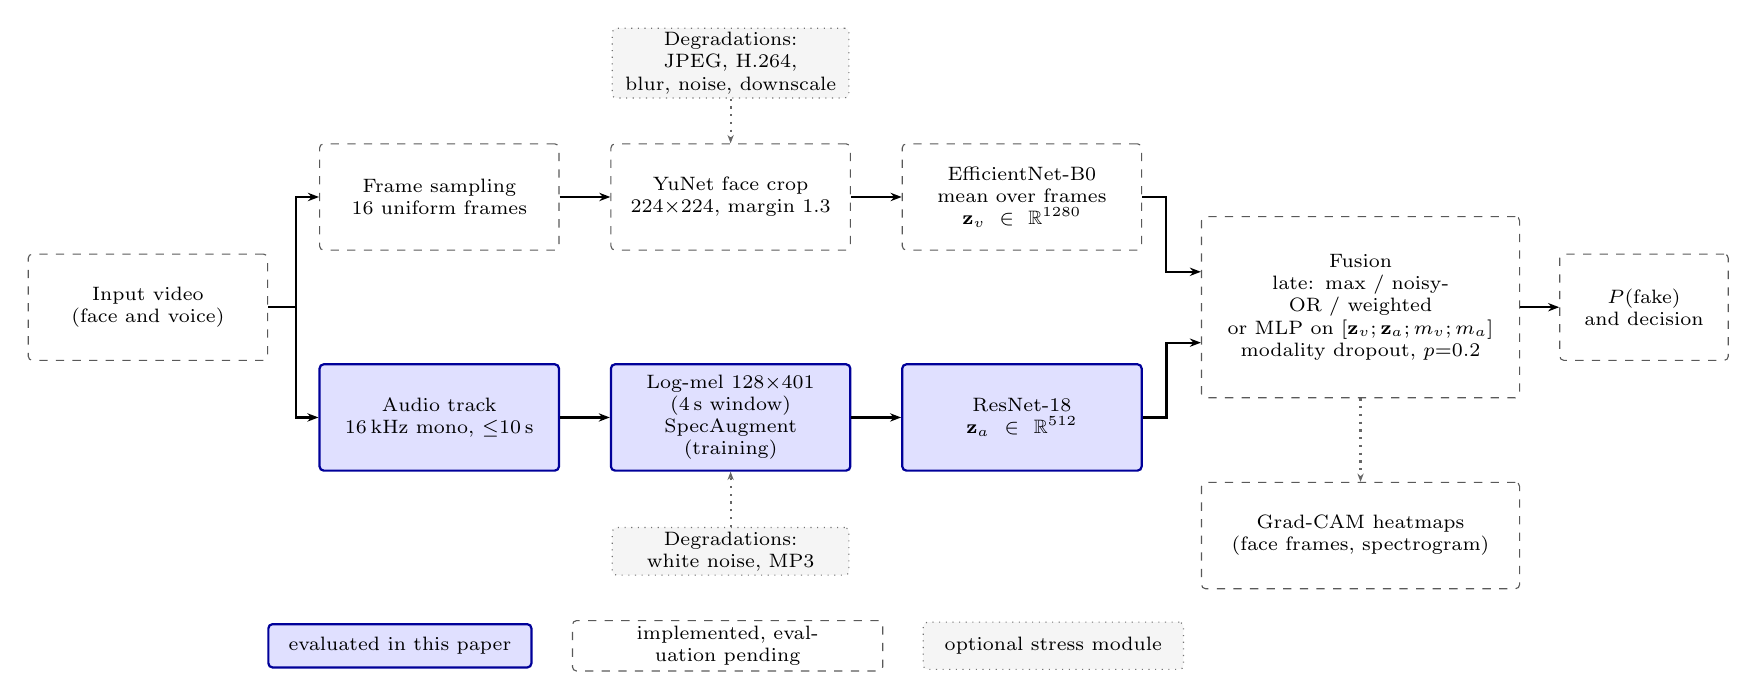
\begin{tikzpicture}[
  font=\scriptsize,
  box/.style={draw, rounded corners=1.5pt, minimum height=1.35cm, text width=2.9cm, align=center, inner sep=2pt},
  done/.style={box, fill=blue!12, draw=blue!60!black, thick},
  todo/.style={box, dashed, draw=black!65},
  deg/.style={draw, dotted, rounded corners=1.5pt, text width=2.9cm, align=center, inner sep=1.5pt, minimum height=0.6cm, draw=black!55, fill=black!4},
  arr/.style={-{Stealth[length=4pt]}, thick},
  darr/.style={-{Stealth[length=3pt]}, dotted, thick, black!60}
]
\node[todo] (in)  at (0,0)      {Input video\\(face and voice)};
\node[todo] (fr)  at (3.7,1.4)  {Frame sampling\\16 uniform frames};
\node[todo] (fc)  at (7.4,1.4)  {YuNet face crop\\$224{\times}224$, margin 1.3};
\node[todo] (vb)  at (11.1,1.4) {EfficientNet-B0\\mean over frames\\$\mathbf z_v\in\mathbb R^{1280}$};
\node[done] (au)  at (3.7,-1.4) {Audio track\\16\,kHz mono, $\leq$10\,s};
\node[done] (mel) at (7.4,-1.4) {Log-mel $128{\times}401$\\(4\,s window)\\SpecAugment (training)};
\node[done] (ab)  at (11.1,-1.4) {ResNet-18\\$\mathbf z_a\in\mathbb R^{512}$};
\node[todo, text width=3.9cm, minimum height=2.3cm] (fu) at (15.4,0) {Fusion\\late: max / noisy-OR / weighted\\or MLP on $[\mathbf z_v;\mathbf z_a;m_v;m_a]$\\modality dropout, $p{=}0.2$};
\node[todo, text width=2.0cm] (out) at (19.0,0) {$P(\mathrm{fake})$\\and decision};
\node[deg] (dv) at (7.4,3.1)  {Degradations: JPEG, H.264,\\blur, noise, downscale};
\node[deg] (da) at (7.4,-3.1) {Degradations:\\white noise, MP3};
\node[todo, text width=3.9cm] (gc) at (15.4,-2.9) {Grad-CAM heatmaps\\(face frames, spectrogram)};

\draw[arr] (in.east) -- ++(0.35,0) |- (fr.west);
\draw[arr] (in.east) -- ++(0.35,0) |- (au.west);
\draw[arr] (fr) -- (fc);
\draw[arr] (fc) -- (vb);
\draw[arr] (au) -- (mel);
\draw[arr] (mel) -- (ab);
\draw[arr] (vb.east) -- ++(0.3,0) |- ($(fu.west)+(0,0.45)$);
\draw[arr] (ab.east) -- ++(0.3,0) |- ($(fu.west)+(0,-0.45)$);
\draw[arr] (fu) -- (out);
\draw[darr] (dv) -- (fc);
\draw[darr] (da) -- (mel);
\draw[darr] (fu) -- (gc);

% legend
\node[done, text width=3.2cm, minimum height=0.55cm] (l1) at (3.2,-4.3) {evaluated in this paper};
\node[todo, text width=3.8cm, minimum height=0.55cm, right=0.5cm of l1] (l2) {implemented, evaluation pending};
\node[deg, text width=3.2cm, right=0.5cm of l2] (l3) {optional stress module};
\end{tikzpicture}
\end{document}
